\chapter{Temperature sensor conditioning circuit}\label{sec:temp_sensor}

%**********************************************
\section{Intro} \label{sec:temp_intro}
%**********************************************
The signal obtained from the temperature sensor presents as DC, with \SI{50}{Hz} AC noise superimposed. The sensor output is too small for a ADC to take as input. Furthermore, the applicable range is only from 34\degree C to 42\degree C. The two aforementioned considerations necessitate amplification of the relevant part of the temperature sensor signal to a \numrange{0}{5} \si{\volt} range for an ADC. To this end, a temperature sensor conditioning circuit is required, making use of a filter, an offset removing subcircuit, as well as an amplifier. The filter attenuates the AC signal present in the input signal in order to minimize noise. The offset removing subcircuit removes enough of the DC offset to ensure that the output signal is centered around \SI{2.5}{\volt}, to ensure the largest possible output swing. Finally, the amplifier increases the magnitude of the input signal in order to be suitable as input for an ADC.

%**********************************************
\section{Design}\label{sec:temp_design}
%**********************************************
The amplifier was designed first, as its gain serves as the determining factor for the amount of noise reduction that is required from the filter. A TLC2272 op-amp was chosen as it allows for an output very close to its rails. Since the output signal has to be centered around \SI{2.5}{\volt}, a differential amplifier was decided upon, as the negative input can adjust the output offset. The zero-reference temperature sensor voltage ($V_{zero}$) is \SI{440}{\milli \volt}, and increases by \SI{35}{\milli \volt} for every 1\degree C ($V_{\Delta}$). Therefore  $V_{temp} = V_{zero} + V_{\Delta} \times \mathrm{Temp}$. As shown in table \ref{tab:temp}, the maximum 

\begin{wraptable}{R}{0.65\textwidth}
%\begin{table}[h]
        \centering
%        \vspace{-2cm}
        \footnotesize
        \caption{Temperatures and Corresponding Voltage Levels}
         \begin{tabular}{c@{\qquad}rrr}
          \toprule
          Temperature [\degree C] 	& 32    & 38	& 42\\
          Voltage [V] 			& 1.63	& 1.77	& 1.91\\
          \bottomrule
        \end{tabular}
     \label{tab:temp}
%\end{table}
\end{wraptable}

input voltage swing equals $1.91 - 1.63 = 0.28$V, and has a DC offset of \SI{1.77}{\volt}. Amplification is needed to reach an output voltage swing of \SI{5}{\volt}, which, combined with a \SI{2.5}{V} DC offset, will ensure that the circuit uses the input range as specified, and excludes the lower and upper temperature ranges (i.e. below 34\degree C and above 42\degree C). Therefore:

$$A_v = \frac{V_{out}}{V_{in}} = \frac{5}{0.28} = 17.86$$

Considering the current design requirement of \SI{25}{mA} maximum, the input resistor R is selected as \SI{10}{\kilo \Omega}, which will therefore, at the highest possible voltage level (\SI{5}{\volt}), use \SI{0.5}{mA} of current.  This gives $R_{feedback} = 178.6$k$\Omega$, according to $A_v = \frac{{R}_{feedback}}{R}$ \cite{opamp}. R corresponds to $R_1$ and $R_2$, and $R_{feedback}$ to $R_{3}$ and $R_4$ in the final design diagram (figure \ref{fig:final}), which is shown here already to aid with the explanation of the design process. 

\begin{figure}[H]
    \centering
    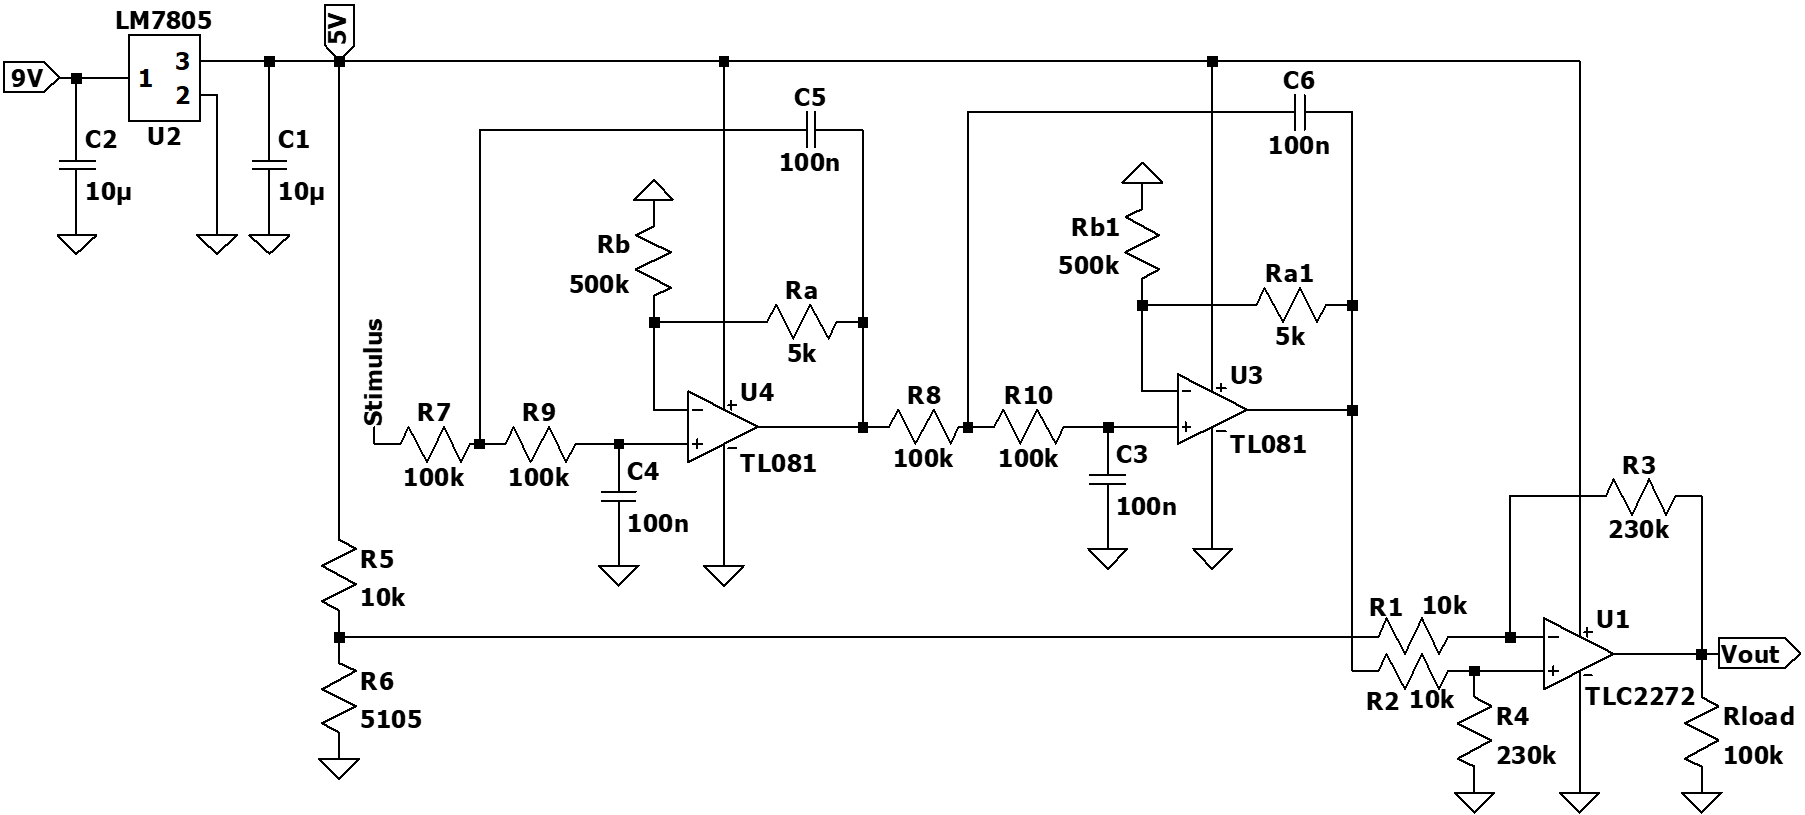
\includegraphics[width = 1\textwidth]{Figures/final.png}
    \caption{Temperature Sensor Circuit}
    \label{fig:final}
\end{figure}

Two points need to be considered: 
\begin{enumerate}
\item The DC offset of the input signal is undesired and has to be removed in order to obtain a zero-mean input signal. This can be achieved by designing another subcircuit that makes use of another op-amp, for example. This adds to the cost and complexity of the circuit.
\item The output signal has to be centered around \SI{2.5}{\volt}. This means that a DC offset has to be added in the form of a virtual ground.
\end{enumerate}

When considered in conjunction with each other, the DC offset alteration can be resolved in one step, thereby reducing cost and complexity significantly. The decision was therefore made to use a differential amplifier, with the input signal connected to the positive input, after which the voltage required at the negative input can be calculated in such a way as to simultaneously subtract the offset and add the virtual ground in one step, thereby producing an output DC offset of \SI{2.5}{\volt}.  This approach also simplifies the design procedure, as it becomes unnecessary to calculate the virtual ground separately (the lecturer mentions that this is an acceptable approach in Lecture Video 2, minute 11\cite{vground}; this removes the need to perform any virtual ground calculations per se - feel free to double-check with the lecturer). The differential amplifier, however, has to be non-inverting. The calculation thus reduces to a simple differential amplifier gain formula \cite{opamp}: 

$$V_{out}=\frac{{R}_{feedback}}{{R}}\left({V}_{in+}-{V}_{in-}\right) \;\;\; \rightarrow \;\;\; 2.5=\frac{178600}{10000}\left(1.77-{V}_{in-}\right)$$

With $V_{out}$ as \SI{2.5}{\volt}, $V_{in+}$ as \SI{1.77}{\volt} and the resistor values as calculated previously, ${V}_{in-} = 1.63 \; \mathrm{V}$. The voltage at ${V}_{in-}$ can be set by means of a voltage divider circuit, which takes \SI{5}{\volt} as input and is calculated as follows (resistor names in formulae are selected to conform with Figure \ref{fig:final}): ${V}_{in-} = 5 (\frac{R_{6}}{R_{6}\times R_{5}})$. Selecting $R_5$ as \SI{10}{\kilo \Omega} gives $R_6 =$ \SI{4.84}{\kilo \Omega}. Here, the common-mode voltage, $V_{IC}$, needs consideration; the TLC2272 can operate with a common-mode voltage of $V_{DD-}$ to $V_{DD+} - 1.5$\cite{tlc}. Since $V_{{in+}_{max}}$ is \SI{1.91}{\volt} and $V_{in-}$ is \SI{1.63}{\volt}, the largest possible common mode voltage is $V_{IC} = \frac{1.91 + 1.63}{2} =$ \SI{1.77}{\volt}, which is well below the maximum limit. Since $V_{in-}$ stays constant, the lower limit will never be reached either.\\

Simulation was used to select a filter, and has shown the following: the RC filter is very simple, but produces too much noise. The passive low-pass filter is relatively simple, but does not meet the settling time requirement. The active low-pass filter meets both the noise and settling time requirements, but requires the TLC2272 op-amp to do so. Since a single TLC2272 op-amp is more expensive than multiple TL081 op-amps, the decision was made to rather use cascaded second order low-pass filters, which  make use of the TL081. This is somewhat more complex, but lowers the cost, as the final circuit now only uses three op-amps, two of which are the cheaper TL081 models. The cascaded setup also produces an output signal with extremely low noise.  A filter gain of close to unity is desired; for $R_A = $ \SI{500}{\kilo\Omega}, a value of \SI{5}{\kilo\Omega} is suitable for $R_A$, according to the formula\cite{filter}: ${A_v}=1+\frac{{R}_A}{R_B}$

The settling time requirement of \SI{100}{ms} means that a cutoff frequency of more than \SI{10}{Hz} is needed, while the attenuation of noise requires a cutoff frequency below \SI{50}{Hz}. $f_c = $ \SI{15}{Hz} was chosen - the bandwidth thus also is \SI{15}{Hz}. Choosing R ($\mathrm{R_7 \; and \; R_9}$ in the diagram) as \SI{100}{\kilo\Omega} gives C ($\mathrm{C_4 \; and \; C_5}$) as \SI{106.1}{nF}, according to $f_c=\frac{1}{2 \pi RC}$. The given cutoff frequency implies a rise time of \SI{19.1}{ms} according to $t_{r} \approx \frac{1.8}{w_{n}} = \frac{1.8}{2 \pi (15)}$\cite{cs}. This meets the requirement of \SI{100}{ms}. After design completion, this filter is then duplicated and connected back-to-back in order to form cascaded second-order low-pass filters, as seen in figure \ref{fig:final}.\\

Using the assumption that each resistor is subjected to an average voltage of \SI{2.5}{\volt}, while the op-amp draws 3 mA\cite{tlc}, the total temperature sensor current consumption is: 

$I_{temp} = (2)\frac{2.5}{10k} + (2)\frac{2.5}{178.6k} + 3mA = 3.53mA$

and the calculated current for the total circuit is:

$I_{total} = (3)\frac{2.5}{10k} + (2)\frac{2.5}{178.6k} + (4)\frac{2.5}{100k} + (2)\frac{2.5}{500k} + (3)\frac{2.5}{5k} + (2)\frac{2.5}{178.6k} + (3)3mA = 11.39mA$

 
%**********************************************
\section{Results} \label{sec:temp_results}
%**********************************************
The designed circuit receives an input signal ranging from 1.67 to \SI{1.94}{\volt} for $V_{in+}$, which is somewhat higher than the calculated values of 1.63 to \SI{1.91}{\volt}, and is due to the filter adding some offset. This can easily be overcome by adjusting the voltage divider. $V_{in-}$ receives \SI{1.7}{\volt}. Both $V_{in-}$ and $V_{in+}$ thus fall well within the allowable range for the TLC2272, which is from $\mathrm{V}_{\mathrm{DD}-}-0.3 \;\; \mathrm{to} \;\; \mathrm{V}_{\mathrm{DD}+}$\cite{tlc}.  The circuit produces a signal centered at \SI{2.5}{\volt} with an output swing of \SI{4.86}{\volt} (figure \ref{subfig:vout}), exceeding the required \SI{3.5}{\volt}. The absolute maximum amount of noise measured is \SI{25.6}{\milli\volt} (figure \ref{subfig:noise}), and the settling time is \SI{67}{ms} (figure \ref{subfig:ts}), thereby meeting the requirements of \SI{50}{\milli\volt} and \SI{100}{ms} respectively. Total current draw is \SI{12.83}{mA} (figure \ref{subfig:current}), well below the required \SI{15}{mA}, and very close to the calculated \SI{11.39}{mA}. The cutoff frequency, obtained via AC analysis simulation, is \SI{10.48}{Hz} (figure \ref{fig:ac}). Measurements and graphs of settling time, cutoff frequency and current drawn can be seen in Appendix C. It is thus clear that all requirements, as well as all bonus requirements, have been met with a good margin to spare, all the while using only three op-amps, two of which are the cheaper TL081 models. The output signal (light blue) is shown in figure \ref{subfig:vout}.

\begin{figure}[h]
 \footnotesize
 \centering
    \begin{subfigure}[]{0.45\textwidth}
              \centering
  		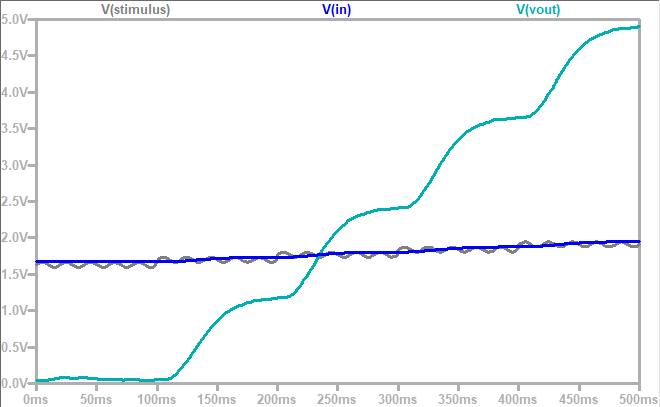
\includegraphics[width=1\linewidth]{./Figures/vout}
		    \caption{Full Input and Output Range} \label{subfig:vout}
     \end{subfigure}
     \begin{subfigure}[]{0.45\textwidth}
             \centering
  		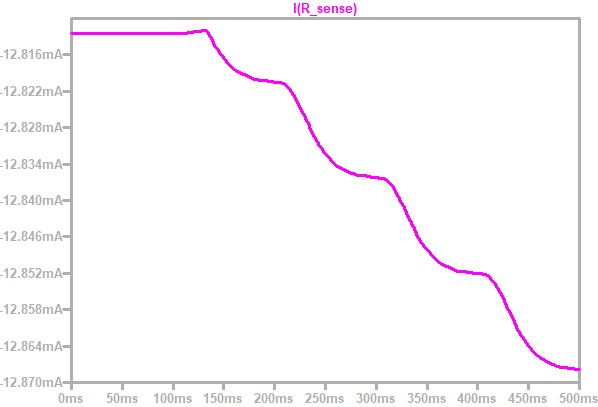
\includegraphics[width=1.0\linewidth]{./Figures/current}
		   \caption{Total Current of Entire System} \label{subfig:current}
     \end{subfigure}
    \begin{subfigure}[]{0.45\textwidth}
              \centering
  		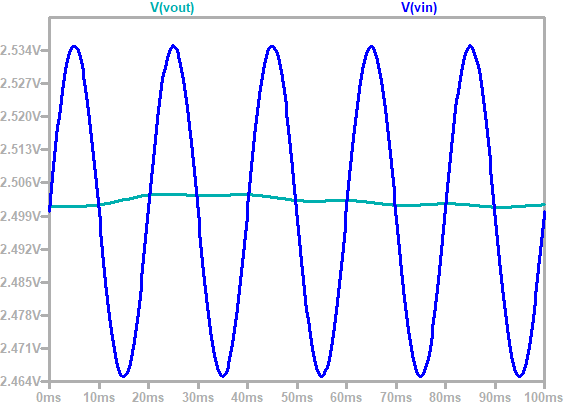
\includegraphics[width=1\linewidth]{./Figures/noise}
		    \caption{Simulated Noise Suppresion} \label{subfig:noise}
     \end{subfigure}
    \begin{subfigure}[]{0.45\textwidth}
              \centering
  		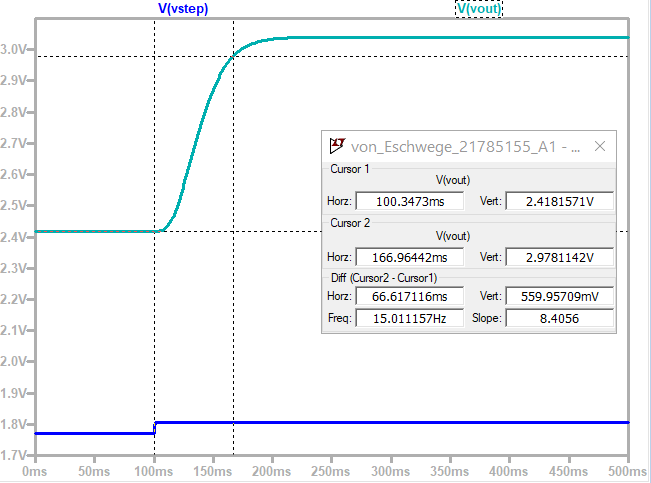
\includegraphics[width=1\linewidth]{./Figures/ts}
		    \caption{Simulated Output Rise Time} \label{subfig:ts}
     \end{subfigure}
   \caption[\textcolor{red}{Complete Circuit Output}]{Complete Circuit Output (a) Output Range: 0.1 to 4.85V. Input Range: 1.63 to 1.94 V. (b)  Current draw below requirement.  (c)  Noise suppressed to negligible levels. (d) Settling time within 100 ms.}
    \label{fig:simulation_results_box}
 \end{figure}

%**********************************************
\section{Summary}\label{sec:temp_summary}
%**********************************************
Concluding, the circuit performs very well, and successfully amplifies the temperature sensor output to a level that is readable by the microcontroller ADC, all the while attenuating almost all noise present in the input. The design is somewhat complex, but also cheaper, as it uses less of the TLC2272 op-amps. It meets all requirements and bonus requirements.


